\documentclass{beamer}
\usetheme[numbering=progressbar]{focus}
\usepackage{tikz}
\usetikzlibrary{positioning}
\usetikzlibrary{shapes,arrows}
\usepackage{transparent}
\usepackage{fancyvrb}
\usepackage{listings}
\definecolor{main}{RGB}{47, 161, 219}
%\definecolor{textcolor}{RGB}{128, 128, 128}
\definecolor{background}{RGB}{240, 247, 255}
\definecolor{textcolor}{RGB}{85, 87, 83}
\title{Improving Passive DNS collection}
\subtitle{with D4 Project}
\author{Alexandre Dulaunoy}
\titlegraphic{
\includegraphics[scale=0.20]{d4-logo.pdf}}
\institute{Team CIRCL \\ \url{https://www.d4-project.org/}}
\date{2019/03/29}

\begin{document}
    \begin{frame}
        \maketitle
    \end{frame}

\begin{frame}
        \frametitle{Problem statement}
        \begin{itemize}
                \item CIRCL (and other CSIRTs) have their own passive DNS\footnote{\url{https://www.circl.lu/services/passive-dns/}} collection mechanisms
                \item Current {\bf collection models} are affected with DoH\footnote{DNS over HTTPS} and centralised DNS services
                \item DNS answers collection is a tedious process
                \item {\bf Sharing Passive DNS stream} between organisation is challenging due to privacy
        \end{itemize}
\end{frame}


\begin{frame}
        \frametitle{Potential Strategy}
 \begin{itemize}
         \item Improve {\bf Passive DNS collection diversity} by being closer to the source and limit impact of DoH (e.g. at the OS resolver level)
         \item Increasing diversity and {\bf mixing models} before sharing/storing Passive DNS records
         \item Simplify process and tools to install for {\bf Passive DNS collection by relying on D4 sensors} instead of custom mechanisms
         \item Provide a distributed infrastructure for mixing streams and filtering out the sharing to the validated partners
 \end{itemize}
\end{frame}

\begin{frame}
        \frametitle{First release}
 \begin{itemize}

         \item analyzer-d4-passivedns\footnote{\url{https://github.com/D4-project/analyzer-d4-passivedns}} is an analyzer for a D4 network sensor. The analyser can process data produced by D4 sensors (in passivedns CSV format\footnote{\url{https://github.com/gamelinux/passivedns}})
         \item Ingest these into a {\bf Passive DNS server} which can be queried later to search for the Passive DNS records
\item The lookup server (using on redis-compatible backend) is a Passive DNS REST server compliant to the Common Output Format\footnote{\url{https://tools.ietf.org/html/draft-dulaunoy-dnsop-passive-dns-cof-04}}
\end{itemize}
\end{frame}

\begin{frame}
\frametitle{D4 Overview}
        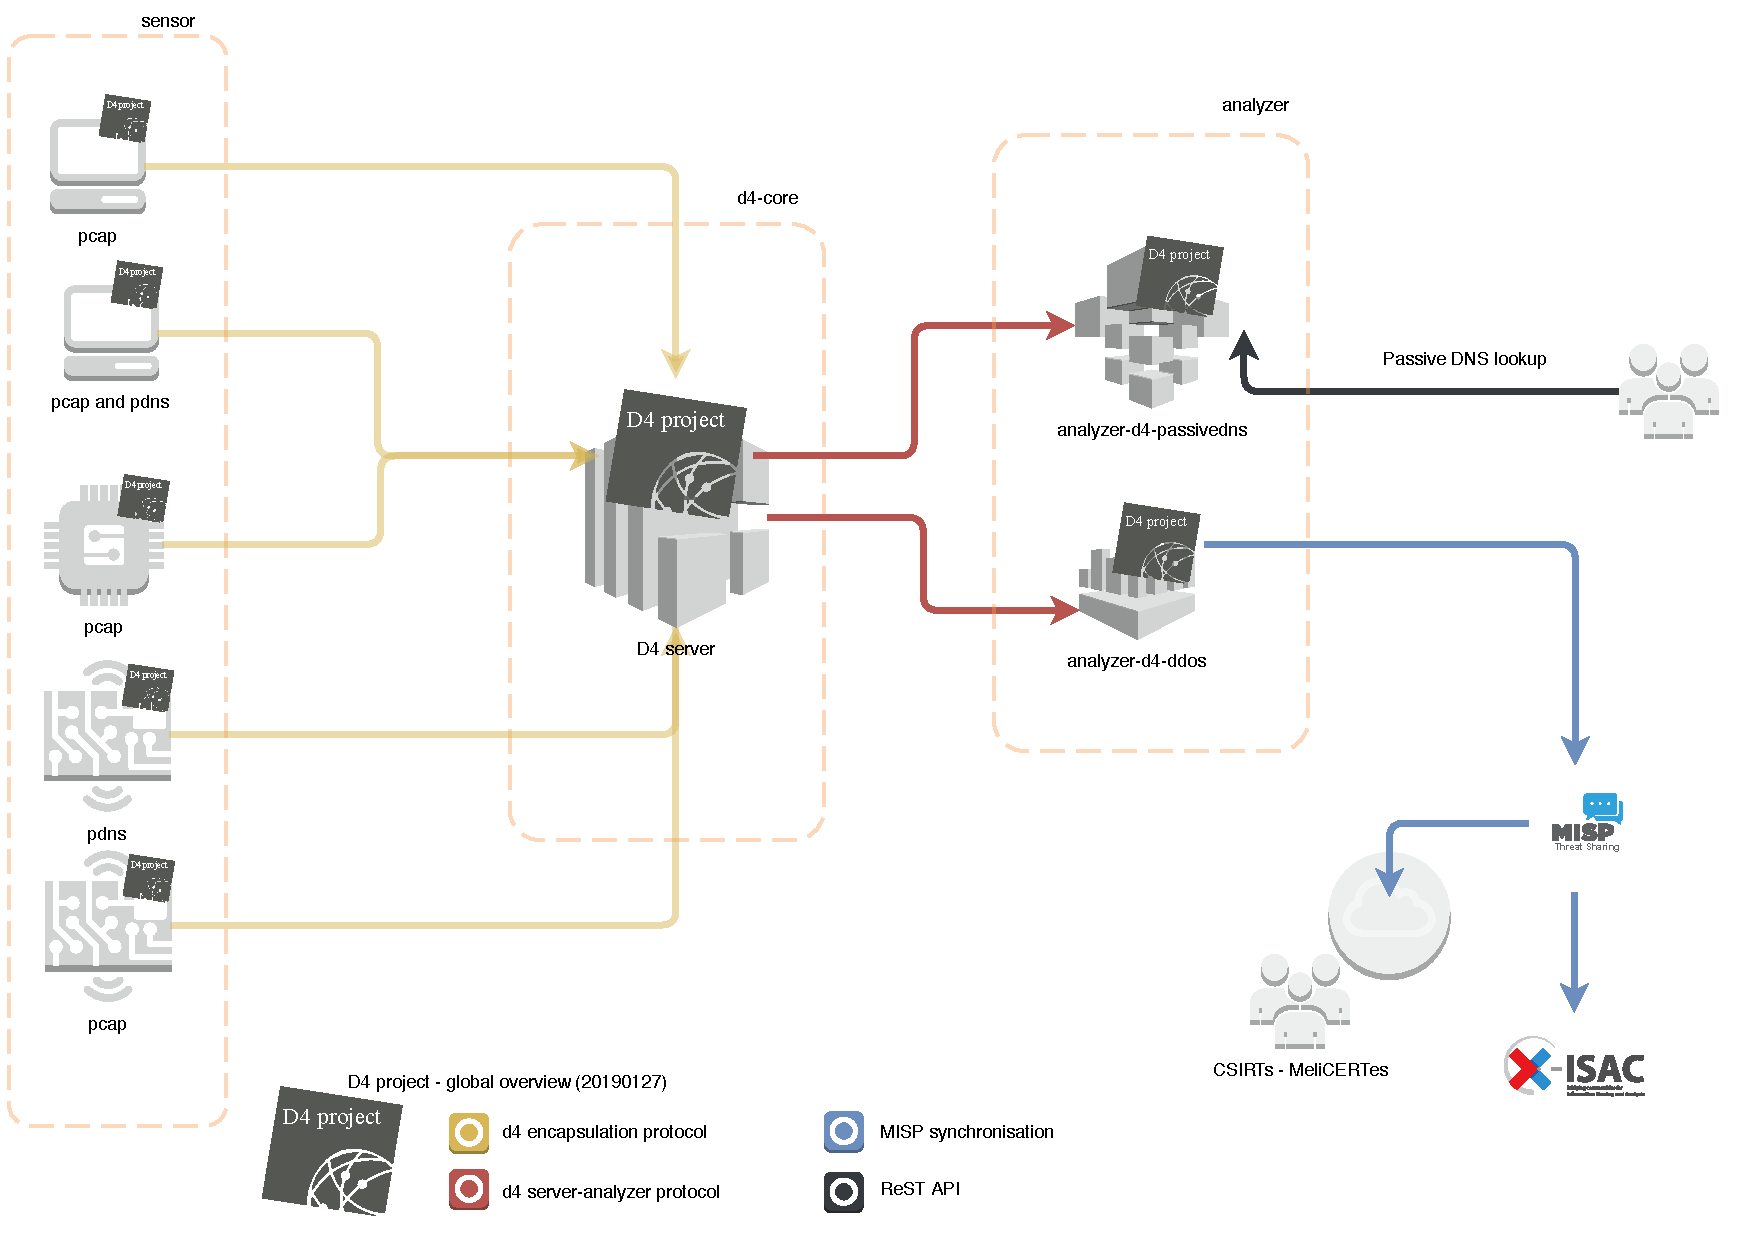
\includegraphics[scale=0.38]{d4-overview.pdf}
\end{frame}


\begin{frame}[t]{Common Output Format}
\begin{itemize}
\item {\bf Consistent naming of fields across Passive DNS software} based on the most common Passive DNS implementations
\item Minimal set of fields to be supported
\item Minimal set of optional fields to be supported
\item Way to add "additional" fields via a simple registry mechanism (IANA-like)
\item Simple and easily parsable format
\item A gentle reminder regarding privacy aspects of Passive DNS
\end{itemize}
\end{frame}

\begin{frame}[t,fragile]{Sample output www.terena.org}
\lstdefinelanguage{JavaScript}{
  keywords={typeof, new, true, false, catch, function, return, null, catch, switch, var, if, in, while, do, else, case, break},
  keywordstyle=\color{blue}\bfseries,
  ndkeywords={class, export, boolean, throw, implements, import, this},
  ndkeywordstyle=\color{darkgray}\bfseries,
  identifierstyle=\color{black},
  sensitive=false,
  comment=[l]{//},
  morecomment=[s]{/*}{*/},
  commentstyle=\color{purple}\ttfamily,
  stringstyle=\color{red}\ttfamily,
  morestring=[b]',
  morestring=[b]"
}

\lstset{
   language=JavaScript,
   backgroundcolor=\color{lightgray},
   extendedchars=true,
   basicstyle=\footnotesize\ttfamily,
   showstringspaces=false,
   showspaces=false,
   numbers=left,
   numberstyle=\footnotesize,
   numbersep=9pt,
   tabsize=2,
   breaklines=true,
   showtabs=false,
   captionpos=b
}
\lstset{breaklines=true, language=JavaScript}
\begin{lstlisting}
{"count": 868, "time_first": 1298398002, "rrtype": "A", "rrname": "www.terena.org", "rdata": "192.87.30.6", "time_last": 1383124252}
{"count": 89, "time_first": 1383729690, "rrtype": "CNAME", "rrname": "www.terena.org", "rdata": "godzilla.terena.org", "time_last": 1391517643}
{"count": 110, "time_first": 1298398002, "rrtype": "AAAA", "rrname": "www.terena.org", "rdata": "2001:610:148:dead::6", "time_last": 136670845}
\end{lstlisting}
\end{frame}


\begin{frame}[t]{Mandatory fields}
\begin{itemize}
\item \textbf{rrname} : name of the queried resource records
\begin{itemize}
\item JSON String
\end{itemize}
\item \textbf{rrtype} : resource record type
\begin{itemize}
\item JSON String (interpreted type of resource type if known)
\end{itemize}
\item \textbf{rdata} : resource records of the query(ied) resource(s)
\begin{itemize}
\item JSON String or an array of string if more than one unique triple
\end{itemize}
\item \textbf{time\_first} : first time that the resource record triple (rrname, rrtype, rdata) was seen
\item \textbf{time\_last} : last time that the resource record triple (rrname, rrtype, rdata) was seen
\begin{itemize}
\item JSON Number (epoch value) UTC TZ
\end{itemize}
\end{itemize}
\end{frame}

\begin{frame}[t]{Optional fields}
\begin{itemize}
\item \textbf{count} : how many authoritative DNS answers were received by the Passive DNS collector
\begin{itemize}
\item JSON Number
\end{itemize}
\item \textbf{bailiwick} : closest enclosing zone delegated to a nameserver served in the zone of the resource records
\begin{itemize}
\item JSON String
\end{itemize}

\end{itemize}
\end{frame}

\begin{frame}[t]{Additionals fields}
\begin{itemize}
\item \textbf{sensor\_id} : Passive DNS sensor information
\begin{itemize}
\item JSON String
\end{itemize}
\item \textbf{zone\_time\_first} : specific first/last time seen when imported from a master file
\item \textbf{zone\_time\_last}
\begin{itemize}
\item JSON Number
\end{itemize}
\item Additional fields can be requested via \url{https://github.com/adulau/pdns-qof/wiki/Additional-Fields}
\end{itemize}
\end{frame}

\begin{frame}[t]{Future}
\begin{itemize}
        \item {\bf Mixing models for passive DNS stream} (for privacy) in next version of D4 core server
        \item Interconnecting private D4 sensor networks with other D4 sensor networks (sharing to partners filtered stream)
        \item Previewing dataset collected in D4 sensor network and providing {\bf open data stream} (if contributor agrees to share under specific conditions)
\end{itemize}

\end{frame}


\begin{frame}
\frametitle{Get in touch if you want to join/support the project, host a passive dns sensor or contribute}
\begin{itemize}
\item Collaboration can include research partnership, sharing of collected streams or improving the software.
\item Contact: info@circl.lu
\item \url{https://github.com/D4-Project} -  \url{https://twitter.com/d4_project}
\end{itemize}
\end{frame}


\end{document}
